\documentclass{article}

\usepackage{amsmath}
\usepackage{amsthm}
\usepackage{amssymb}
\usepackage{bbm}
\usepackage{fancyhdr}
% \usepackage{listings}
\usepackage{cite}
\usepackage{graphicx}
\usepackage{enumitem}
\usepackage{courier}
\usepackage{framed}

\usepackage[pdftex,colorlinks=true, urlcolor = blue]{hyperref}


\oddsidemargin 0in \evensidemargin 0in
\topmargin -0.5in \headheight 0.25in \headsep 0.25in
\textwidth 6.5in \textheight 9in
\parskip 6pt \parindent 0in \footskip 20pt

% set the header up
\fancyhead{}
\fancyhead[L]{Stanford Aeronautics \& Astronautics}
\fancyhead[R]{Fall 2020}

%%%%%%%%%%%%%%%%%%%%%%%%%%
\renewcommand\headrulewidth{0.4pt}
\setlength\headheight{15pt}

\usepackage{xparse}
\NewDocumentCommand{\codeword}{v}{%
\texttt{\textcolor{blue}{#1}}%
}

\usepackage{xcolor}
\setlength{\parindent}{0in}

\title{AA 274A: Principles of Robot Autonomy I \\ Problem Set 1}
\author{Name: Parthiv Krishna \\ SUID: 06330692}
\date{}

\begin{document}

\maketitle
\pagestyle{fancy} 

\section*{Problem 1: Trajectory Generation via Differential Flatness}
\begin{enumerate}[label=(\roman*)]
\item Given that 
$$x(t)=\sum_{i=1}^{4}x_i\psi_i(t) \text{ and } y(t)=\sum_{i=1}^{4}y_i\psi_i(t)$$ 
and our equations for the $\psi_i(t)$ basis functions, we find that 
$$x(t)=x_1 + x_2t + x_3t^2 + x_4t^3 \text{ and } y(t)=y_1 + y_2t + y_3t^2 + y_4t^3$$ 
From here, we can plug in our known values for $x(0), x(t_f)=x(15), y(0), \text{ and } y(t_f)=y(15)$ to find the first four of our linear equations.
$$x(0) = 0 = x_1$$
$$x(t_f) = x(15) = 5 = x_1 + 15x_2 + 225x_3 + 3375x_4$$
$$y(0) = 0 = y_1$$
$$y(t_f) = y(15) = 5 = y_1 + 15y_2 + 225y_3 + 3375y_4$$
Next, we can differentiate each of the equations for $x(t)$ and find that 
$$\dot{x}(t) = x_2 + 2x_3t + 3x_4t^2 \text{ and } \dot{y}(t) = y_2 + 2y_3t + 3y_4t^2$$
Knowing that $\dot{x}(t) = V(t)\cos(\theta(t))$, we find that 
$$\dot{x}(0) = 0.5\cos(-\pi/2) = 0$$
$$\dot{x}(t_f)=\dot{x}(15)=0.5\cos(-\pi/2) = 0$$ 
Knowing that $\dot{y}(t) = V(t)\sin(\theta(t))$, we find that
$$\dot{y}(0) = 0.5\sin(-\pi/2) = -0.5$$ 
$$\dot{y}(t_f)=\dot{y}(15)=0.5\sin(-\pi/2) = -0.5$$
Now, we have our eight equations for the eight unknowns $x_1 ... x_4$ and $y_1 ... y_4$

\begin{framed}
$$x(0) = 0 = x_1$$ 
$$y(0) = 0 = y_1$$
$$\dot{x}(0) = 0 = x_2$$
$$\dot{y}(0) = -0.5 = y_2$$
$$x(t_f) = x(15) = 5 = x_1 + 15x_2 + 225x_3 + 3375x_4$$
$$y(t_f) = y(15) = 5 = y_1 + 15y_2 + 225y_3 + 3375y_4$$
$$\dot{x}(t_f) = \dot{x}(15) = 0 = x_2 + 30x_3 + 675x_4$$
$$\dot{y}(t_f) = \dot{y}(15) = -0.5 = y_2 + 30y_3 + 675y_4$$
\end{framed}

\item If we set $V(t_f) = 0$, then our matrix J, where both of the right entries have a factor of V, will have a right column of two zeroes. As a result, $\det(J)$ will be zero and J is therefore not invertible, meaning that we cannot find the control inputs. Additionally, we will have $\dot{x}(t_f) = \dot{y}(t_f) = 0$ regardless of $\theta(t_f)$, so we will completely lose any information about the final orientation $\theta(t_f)$ of the robot.

\item Implemented \codeword{compute_traj_coeffs}, \codeword{compute_traj}, and \codeword{compute_control} in \\ \codeword{P1_differential_flatness.py}.

\item Implemented \codeword{compute_arc_length}, \codeword{rescale_V}, \codeword{rescale_tau}, and \codeword{rescale_om} in \\ \codeword{P1_differential_flatness.py}.

\item \codeword{differential_flatness.png} is below. \\ 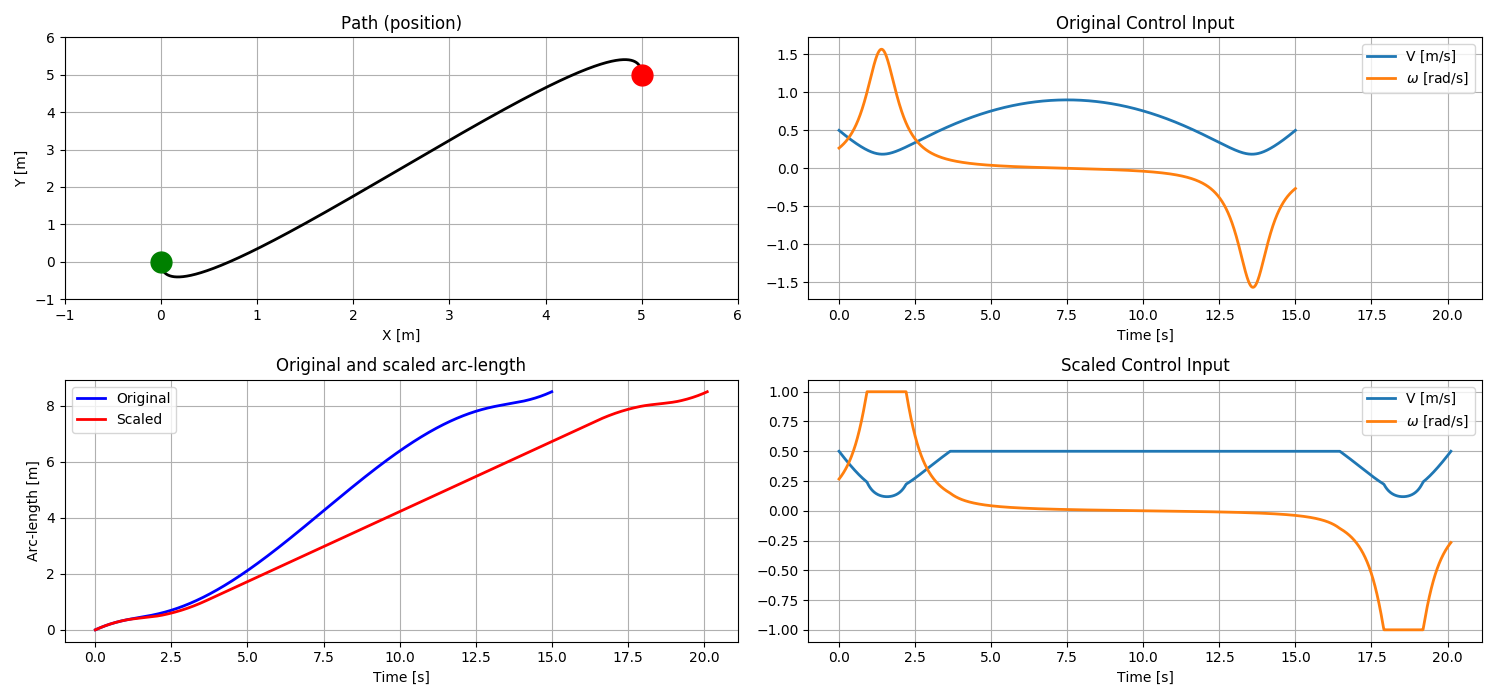
\includegraphics[scale=0.375]{plots/differential_flatness.png}

\item \codeword{sim_traj_openloop.pdf} with the initial conditions in part (i) is below. \\ 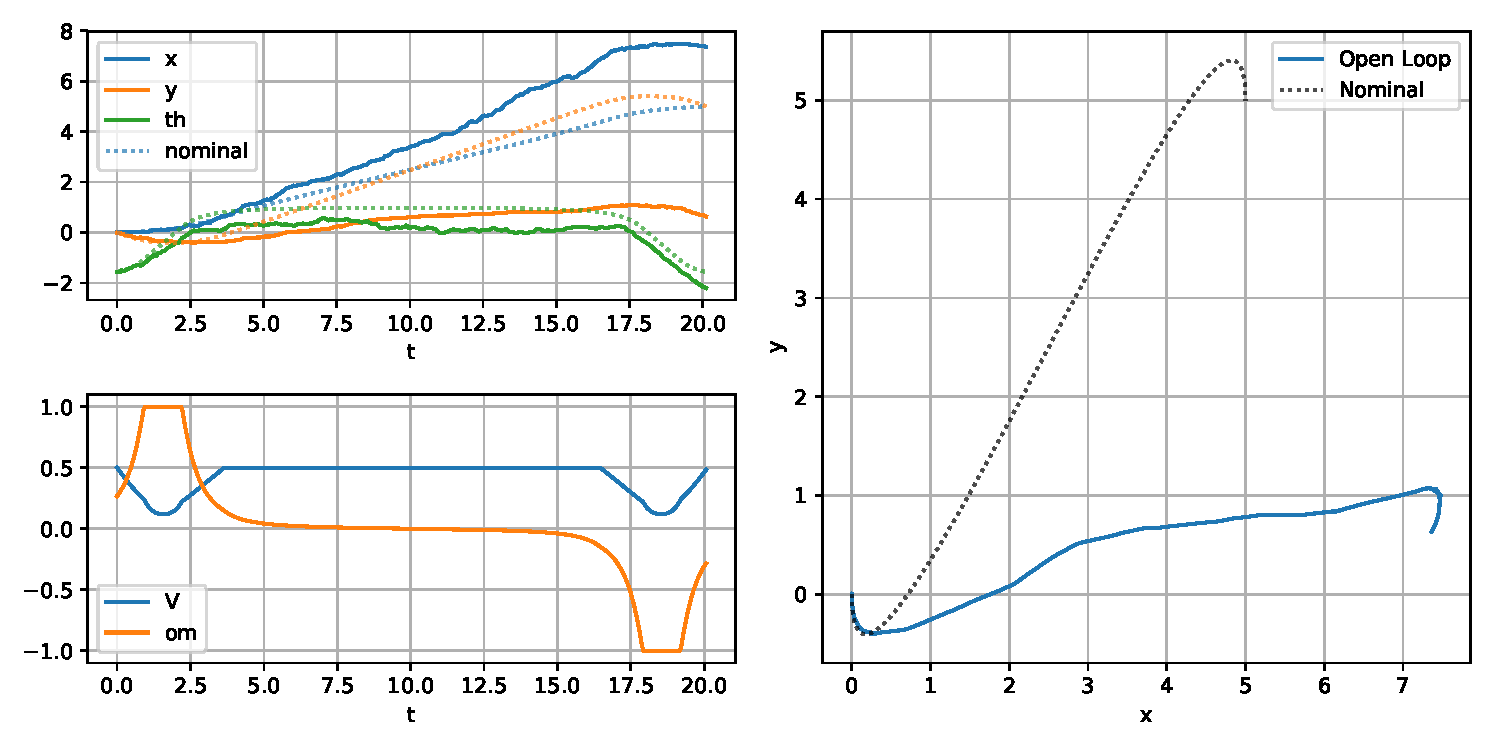
\includegraphics[scale=0.565]{plots/sim_traj_openloop.pdf}

\end{enumerate}

\newpage

\section*{Problem 2: Pose Stabilization}
\begin{enumerate}[label=(\roman*)]
\item Implemented \codeword{compute_control} in the \codeword{PoseController} class in \codeword{P2_pose_stabilization.py}.

\item Validated results with various test configurations.

\item \codeword{sim_parking_forward.png} is below, the robot drives forward and stops. \\
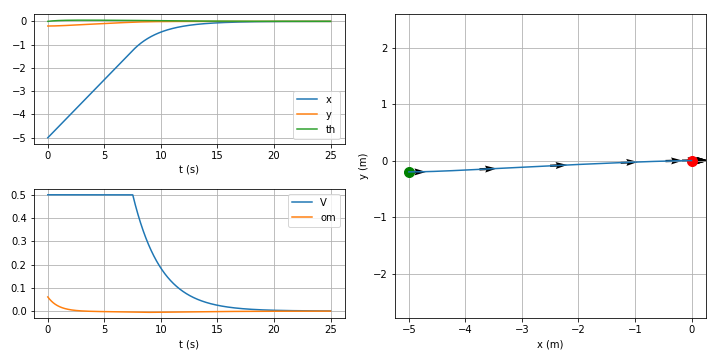
\includegraphics[scale=0.5]{plots/sim_parking_forward.png} \\
\codeword{sim_parking_reverse.png} is below, the robot ends behind the start, facing the start. \\
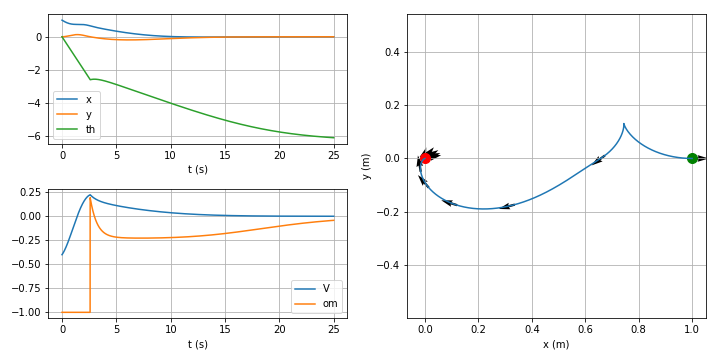
\includegraphics[scale=0.5]{plots/sim_parking_reverse.png} \\
\codeword{sim_parking_parallel.png} is below, the robot ends to the side of the start, facing the same way. \\
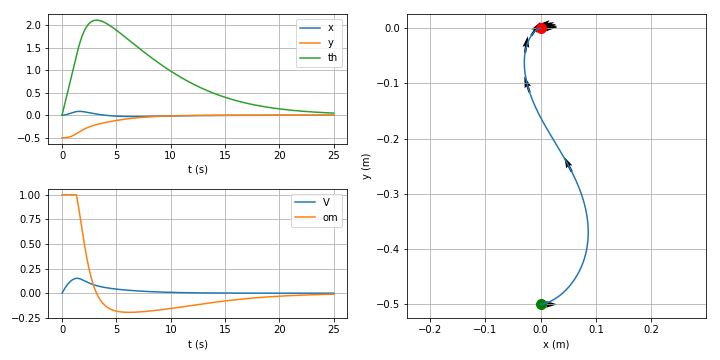
\includegraphics[scale=0.5]{plots/sim_parking_parallel.png}

\end{enumerate}

\newpage

\section*{Problem 3: Trajectory Tracking}
\begin{enumerate}[label=(\roman*)]

\item From the description of Problem 1, we see that

$$\begin{bmatrix}\ddot{x} \\ \ddot{y}\end{bmatrix} = \begin{bmatrix}\cos(\theta) & -V\sin(\theta) \\ \sin(\theta) & V\cos(\theta)\end{bmatrix} \begin{bmatrix} \alpha \\ \omega \end{bmatrix} = \begin{bmatrix}u_1 \\ u_2 \end{bmatrix}$$

% This can be split into two equations.  $u_1 = \ddot{x} = \alpha\cos(\theta) - V\omega\sin(\theta)$ and $u_2 = \ddot{y} = \alpha\sin(\theta) + V\omega\cos(\theta)$. 
In the code, I write this matrix equation as $J\mathbf{x} = \mathbf{u}$, where $\mathbf{x} = \begin{bmatrix}\alpha \\ \omega \end{bmatrix}$. We also know that $\alpha = \dot{V} = \frac{dV}{dt}$. This is our ODE. So we can find $\alpha$ and $\omega$ by first solving $\mathbf{x} = J^{-1}\mathbf{u}$. This gives us $\begin{bmatrix}\alpha \\ \omega \end{bmatrix}$. We can then integrate $\alpha$ numerically to find $V$.

\item Implemented \codeword{compute_control} in the \codeword{TrajectoryTracker} class in \\ \codeword{P3_trajectory_tracking.py}.

\item \codeword{sim_traj_closedloop.pdf} with the initial conditions in part (i) is below. The closed loop controller tracks the desired trajectory quite well, while the open loop controller veers way off the course in the presence of noise. \\ 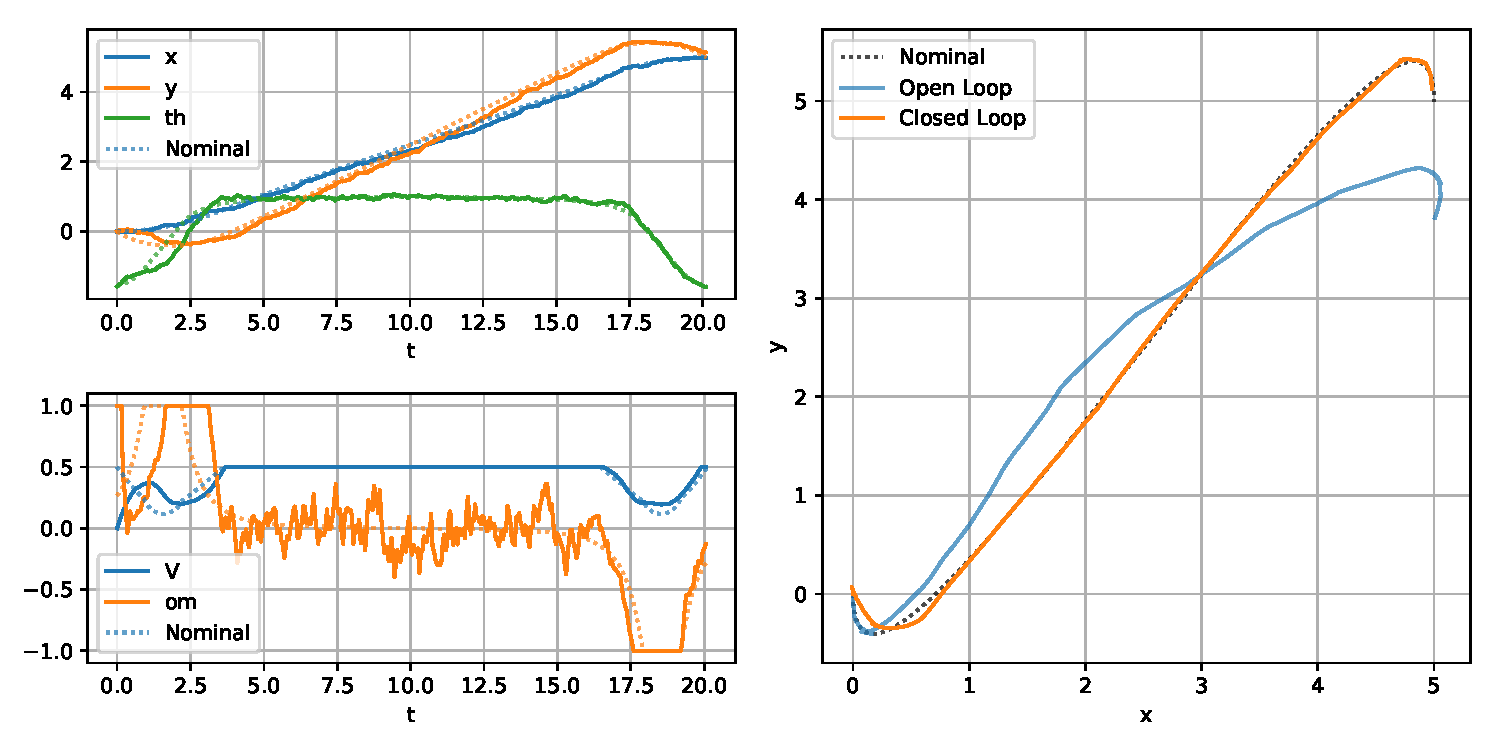
\includegraphics[scale=0.6]{plots/sim_traj_closedloop.pdf}
\end{enumerate}

\newpage

\section*{Extra Problem: Optimal Control and Trajectory Optimization}
\begin{enumerate}[label=(\roman*)]
    \item We want to minimize 
    
    $$J=\int_0^{t_f}[\lambda + V(t)^2 + \omega(t)^2]dt = \int_0^{t_f}g(\mathbf{x}(t), \mathbf{u}(t), t)dt$$
    
    Our robot pose vector is $\mathbf{x}(t) = (x, y, \theta)$. Our control vector is $\mathbf{u}(t) = (V, \omega)$. We we are subject to the dynamics constraints $\mathbf{\dot{x}}(t) = a(\mathbf{x}(t), \mathbf{u}(t), t)$. In this case, we have the standard unicycle constraints:
    $$\dot{x}(t) = V\cos(\theta(t))$$
    $$\dot{y}(t) = V\sin(\theta(t))$$
    $$\dot{\theta}(t) = \omega(t)$$
    
    These three constraints are the three entries of our $a(t)$ function. Therefore, the Hamiltonian is:
    
    $$H(\mathbf{x}(t), \mathbf{u}(t), \mathbf{p}(t), t) = g(\mathbf{x}(t), \mathbf{u}(t), t) + \mathbf{p}^T(t)a(\mathbf{x}(t), \mathbf{u}(t), t)$$
    $$H(\mathbf{x}(t), \mathbf{u}(t), \mathbf{p}(t), t) = \lambda + V(t)^2 + \omega(t)^2 + p_1(t)V\cos(\theta(t)) + p_2(t)V\sin(\theta(t)) + p_3(t)\omega(t)$$
    
    The Necessary Optimality Conditions (NOCs) are given by:
    
    $$\mathbf{\dot{x}}^*(t) = \frac{\partial{H}}{\partial{\mathbf{p}}}(\mathbf{x}^*(t), \mathbf{u}^*(t), \mathbf{p}^*(t), t) $$
    $$\mathbf{\dot{p}}^*(t) = - \frac{\partial{H}}{\partial{\mathbf{x}}}(\mathbf{x}^*(t), \mathbf{u}^*(t), \mathbf{p}^*(t), t) $$
    $$0 = \frac{\partial{H}}{\partial{\mathbf{u}}}(\mathbf{x}^*(t), \mathbf{u}^*(t), \mathbf{p}^*(t), t) $$
    
    In this case, we have the following conditions for optimality:
    \begin{framed}
    $$\begin{bmatrix} \dot{x}^*(t) \\ \dot{y}^*(t) \\ \dot{\theta}^*(t) \end{bmatrix} = \begin{bmatrix} V\cos(\theta(t)) \\ V\sin(\theta(t)) \\ \omega(t)) \end{bmatrix}$$
    $$\begin{bmatrix} \dot{p_1}^*(t) \\ \dot{p_2}^*(t) \\ \dot{p_3}^*(t) \end{bmatrix} = - \begin{bmatrix} 0 \\ 0 \\ -p_1V\sin(\theta(t)) + p_2V\cos(\theta(t)) \end{bmatrix}$$
    $$\mathbf{0} = \begin{bmatrix} 2V(t) + p_1(t)\cos(\theta(t)) + p_2(t)\sin(\theta(t)) \\ 2\omega(t) + p_3(t)\end{bmatrix}$$
    \end{framed}
    From the last equation, we find that 
    $$V(t) = -0.5(p_1(t)\cos(\theta(t)) + p_2(t)\sin(\theta(t)))$$ 
    $$\omega(t) = -0.5p_3(t)$$
    
    \newpage
    The boundary conditions are given by the following, since final state is fixed but final time is free:
    
    $$\mathbf{x}^*(t_0) = \mathbf{x}_0$$
    $$\mathbf{x}^*(t_f) = \mathbf{x}_f$$
    $$H(\mathbf{x}^*(t_f), \mathbf{u}^*(t_f), \mathbf{p}^*(t_f), t_f) + \frac{\partial{h}}{\partial{t}}(\mathbf{x}^*(t_f), t_f) = 0$$
    
    Specifically, in this case, we have the following boundary conditions:
    \begin{framed}
    $$\begin{bmatrix}x(0) - 0 \\ y(0) - 0 \\ \theta(0) + \pi/2 \end{bmatrix} = \mathbf{0}$$
    $$\begin{bmatrix}x(t_f) - 5 \\ y(t_f) - 5 \\ \theta(t_f) + \pi/2\end{bmatrix} = \mathbf{0}$$
    $$\lambda + V(t_f)^2 + \omega(t_f)^2 + p_1(t_f)V\cos(\theta(t_f)) + p_2(t_f)V\sin(\theta(t_f)) + p_3(t_f)\omega(t_f) = 0$$
    \end{framed}
    The first equation provides three left boundary conditions, while the second and third equations provide three and one right boundary conditions respectively. This gives a total of seven boundary conditions, which is the expected $2n+1$ boundary conditions for $n=3$-dimensional pose vector  $\mathbf{x}(t)$.
    
    Finally, to express this whole thing as a 2P-BVP in standard form, we need to find an expression in the form:
    
    $$\dot{\mathbf{z}} = g(\mathbf{z}, t)$$
    $$l(\mathbf{z}(t_0), \mathbf{z}(t_f)) = \mathbf{0}$$
    
    By choosing $\mathbf{z} = (x, y, \theta, p_1, p_2, p_3, t_f)$, we find the following: 
    
    \begin{framed}
    $$\dot{\mathbf{z}} = \begin{bmatrix}\dot{x} \\ \dot{y} \\ \dot{\theta} \\ \dot{p_1} \\ \dot{p_2} \\ \dot{p_3} \\ \dot{t_f}  \end{bmatrix} = \begin{bmatrix} V\cos{\theta} \\ V\sin{\theta} \\ \omega \\ 0 \\ 0 \\ -p_1V\sin(\theta(t)) + p_2V\cos(\theta(t)) \\ 0 \end{bmatrix}$$
    
    $$l(\mathbf{z}(t_0), \mathbf{z}(t_f)) = \begin{bmatrix}x(0) - 0 \\ y(0) - 0 \\ \theta(0) + \pi/2 \\ x(t_f) - 5 \\ y(t_f) - 5 \\ \theta(t_f) + \pi/2 \\ H \end{bmatrix} = \mathbf{0}$$
    
    where $V(t) = -0.5(p_1(t)\cos(\theta(t)) + p_2(t)\sin(\theta(t)))$ 
    $\omega(t) = -0.5p_3(t)$, and the \\ Hamiltonian $H = \lambda + V(t_f)^2 + \omega(t_f)^2 + p_1(t_f)V\cos(\theta(t_f)) + p_2(t_f)V\sin(\theta(t_f)) + p_3(t_f)\omega(t_f)$.
    \end{framed}
    
    \newpage
    
    \item Implemented \codeword{ode_fun}, \codeword{bc_fun}, \codeword{compute_controls}, and \codeword{main} in \codeword{P4_optimal_control.py}. A value of $\lambda = 0.2$ seemed to keep $|V| < 0.5$ and $|\omega| < 1$. The generated trajectory is visibly smooth and takes approximately 17.5 seconds to complete.
    
    \item \codeword{optimal_control.png} is below. \\ 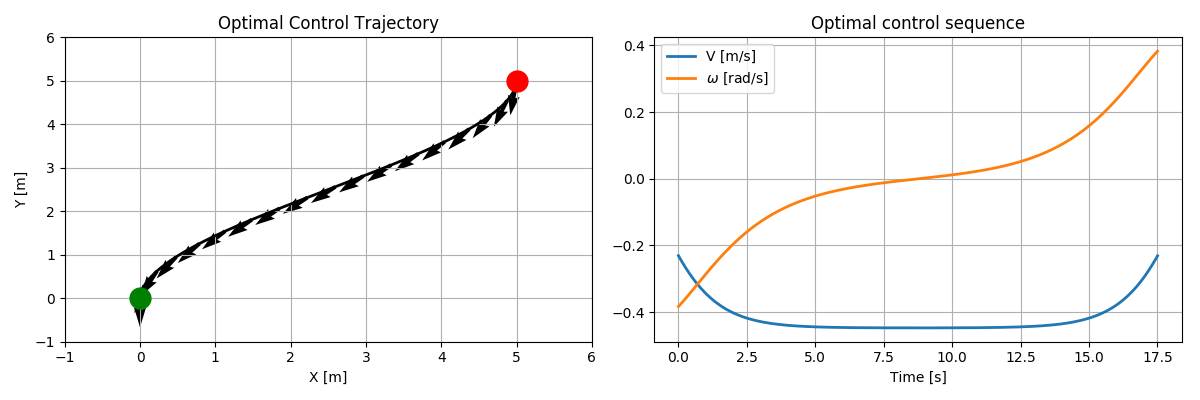
\includegraphics[scale=0.5]{plots/optimal_control.png}
    \\
    When compared to the original trajectory generated by differential flatness in problem 1, this trajectory involves the robot driving backwards (negative V) to more directly reach the goal pose from the initial pose. In the differential flatness trajectory, the robot changes from pointing downwards at start, to pointing upwards/right in cruise, to pointing downwards at the end. With the optimal control approach, the robot completely avoids this behavior of turning around twice, and instead points downwards at the start, downwards/left in cruise, and downwards at the end. This requires less control effort to achieve. Additionally, the plots for $V$ and $\omega$ are much smoother in the optimal control trajectory since we avoid clipping $V$ and $\omega$ by choosing the correct $\lambda$.
    
    \item By using the largest feasible $\lambda$, we minimize the time taken to drive the length of the trajectory (within reason). This is because we are minimizing an integral from $0$ to $t_f$ with $\lambda$ as a constant term within the integrand. So, as $t_f$ increases, the contribution to that integral from the $\lambda$ term increases as well; by making $\lambda$ large, we penalize increases to $t_f$ more.
    
    \item \codeword{sim_traj_optimal_control.pdf} is below.
    
    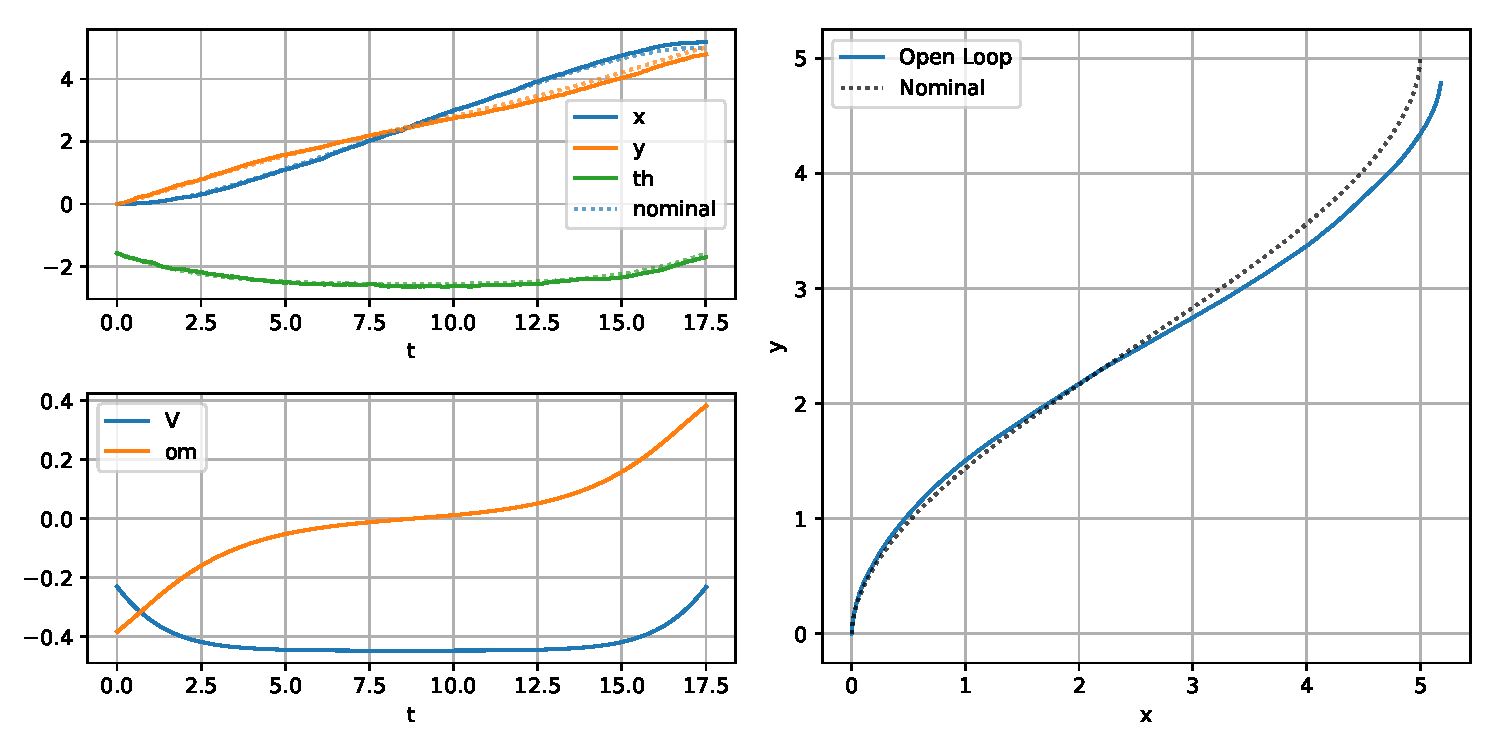
\includegraphics[scale=0.6]{plots/sim_traj_optimal_control.pdf}
    
\end{enumerate}

\end{document}